\documentclass{article}
\usepackage[utf8]{inputenc}
\usepackage{graphicx}

\title{Tugas Pemrograman Chapter3}
\author{Dyah Ayu Anandra (1184098)}
\date{12 Desember 2019}

\begin{document}

\maketitle

\section{Teori}
\subsection{Fungsi pada Python}
\usepackage{Fungsi merupakan bagian dari program yang  memberi statemen dan dapat digunakan ulang. Fungsi dalam Python biasanya menggunakan def sebagai kata kunci. Setelah def kemudian diikut dengan parameter yang tanda kurung dan diakhir dengan tanda titik dua (:). kemudian Baris berikutnya merupakan blok fungsi yang akan dijalankan jika fungsi dipanggil. berikut merupakan contoh sintaks yang digunakan untuk membuat fungsi:}
\begin{itemize}
    \item def function_name(parameters):\\
    """function_docstring"""\\
    statement(s)\\
    return [expression]\\
\end{itemize}

\subsection{Package Python}
\usepackage{Package merupakan sebuah folder tempat menyimpah source kode dan package juga mengelompokkan file python yang telah dibuat yang di dalamnya terdapat fungsi yang telah dibuat.}

\subsection{Class, Object, Atribut, Method}
\begin{enumerate}
    \item Class
    Class merupakan salah satu cara untuk membuat sebuah kode yang mempunyai prilaku tertentu dan lebih mudah dalam mengatur berbagai fungsi. 
    \item Object
    Sebuah objek memiliki variable dan method-nya sendiri dan setiap objek yang dihasilkan akan memiliki karakteristik yang berbeda dengan yang objek lainnya.
    \item Atribut
    Atribut  merupakan  data  atau  fungsi yang  dimiliki  oleh  kelas. Atribut merupakan variabel-variabel  yang  telah  dideklarasikan.
    \item Method
    Method merupakan fungsi yang ada pada sebuah objek ataupun kelas.
\end{enumerate}

\subsection{Pemanggilan Library Kelas dari Instansiasi dan Pemakaiannya Contoh dengan Program}

    \begin{center}
        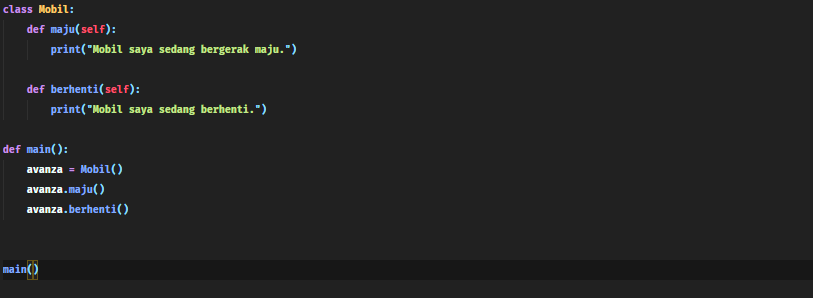
\includegraphics[width = 8cm\textwidth]{F1.png}
    \end{center}
    
\subsection{Pemakaian Paket dengan From kalkulator Import Penambahan}
\usepackage{Conoh:}
\usepackage{from kalkulator import penambahan}
 
 \subsection{Penambahan dari Folder Kalkulator}
 \usepackage{Ketikan terlebih dahulu nama folder Kemudian ketikan import library.}
\usepackage{contoh:}
\usepackage{from library import kelas2}

\section{Keterampilan Pemrograman}
soal 1
\begin{center}
    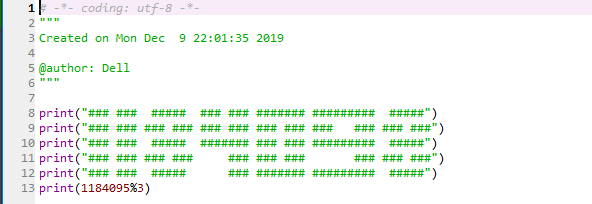
\includegraphics[width = 8cm\textwidth]{a1.png}
\end{center}

soal 2
\begin{center}
    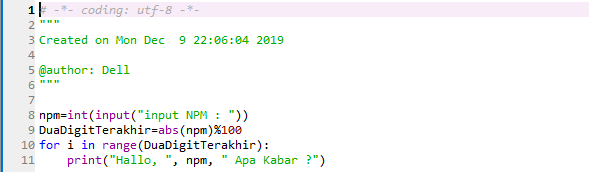
\includegraphics[width = 8cm\textwidth]{a2.png}
\end{center}

soal 3
\begin{center}
    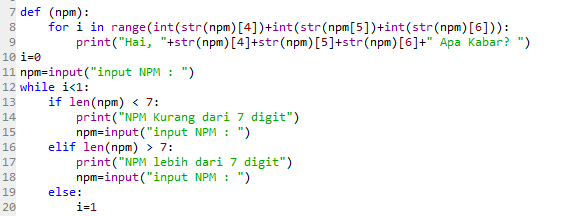
\includegraphics[width = 8cm\textwidth]{aa3.png}
\end{center}

soal 4
\begin{center}
    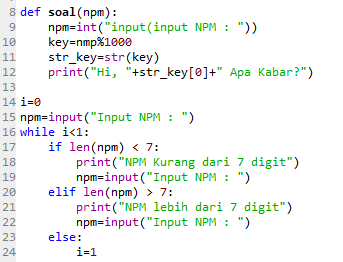
\includegraphics[width = 8cm\textwidth]{aa4.png}
\end{center}

soal 5
\begin{center}
    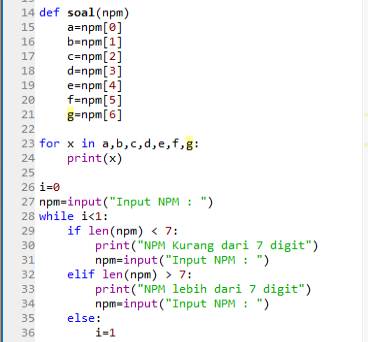
\includegraphics[width = 8cm\textwidth]{aa5.png}
\end{center}

soal 6
\begin{center}
    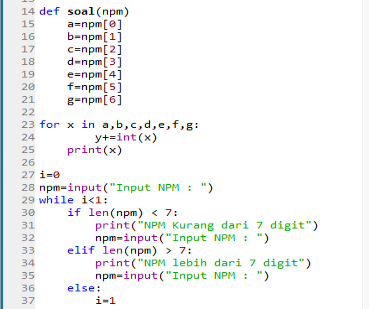
\includegraphics[width = 8cm\textwidth]{aa6.png}
\end{center}

soal 7
\begin{center}
    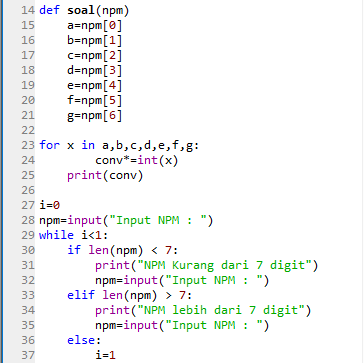
\includegraphics[width = 8cm\textwidth]{aa7.png}
\end{center}

soal 8
\begin{center}
    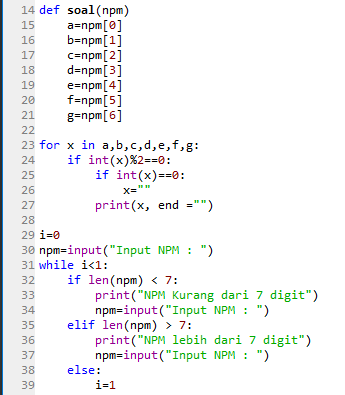
\includegraphics[width = 8cm\textwidth]{aa8.png}
\end{center}

soal 9
\begin{center}
    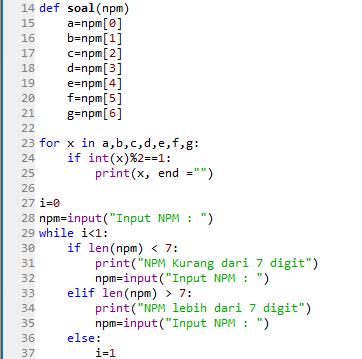
\includegraphics[width = 8cm\textwidth]{aa9.png}
\end{center}

soal 10
\begin{center}
    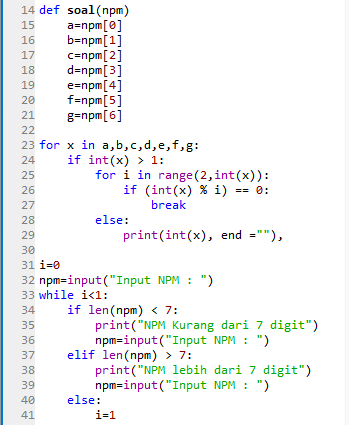
\includegraphics[width = 8cm\textwidth]{aa10.png}
\end{center}

\end{document}
